\documentclass[aspectratio=169,nototalframenumber]{beamer}
\usetheme[nosectiontitlepage]{uibk}

\usepackage{tikz}
\usetikzlibrary{shapes}

\usepackage{graphicx}
\graphicspath{{fig/}}

\title{Enclave-NN State of the Art}
\author{Alexander Schl\"ogl}

\begin{document}

\uibktitlepage{}

\section{Project Concept}
\begin{frame}<1-2>[label=basics]
  \frametitle{Project Concept}
  \begin{center}
    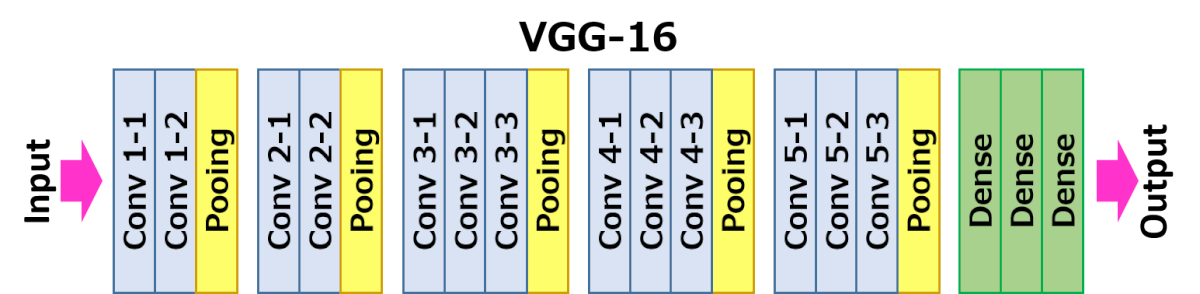
\includegraphics[width=\textwidth]{vgg16.png}
  \end{center}
  
  \pause
  \begin{block}{Model retraining}
    Often only the dense layers are retrained
  \end{block}
  \pause
  \begin{tikzpicture}[overlay,xshift=11.9cm,yshift=3.85cm]
    \node[fill=black!80,text=white,minimum width=1.6cm, minimum height=2.9cm,align=center] (0,0) {TEE};
  \end{tikzpicture}
  
\end{frame}

\section{Motivation}
\begin{frame}
  \frametitle{Motivation}

  ML-as-a-Service works as follows:
  \begin{itemize}
  \item get data from customer
  \item train ML model on their data
  \item charge them per query
  \end{itemize}
  \medskip
  \pause
  \begin{block}{Model privacy}
    In order to monetize you have to keep the model private.\\ 
    This requires that you host the model yourself.
  \end{block}
  \medskip
  \pause
  \begin{block}{Data privacy}
    Customers have to send you their input data for inference.
  \end{block}
\end{frame}

\againframe<3>{basics}

\begin{frame}
  \frametitle{Project Outline}
  \begin{itemize}
  \item Toolchain from ML framework to TEE
  \item Build TEE wrapper for ML framework
  \item Run dense part of VGG-16 in TEE
  \item Collect performance benchmarks
  \item Compare my approach with ML framework
  \item Outlook to \textbf{future work}
  \end{itemize}
\end{frame}

\section{Related Work}
\begin{frame}<1>[label=related]
  \frametitle{Related Work}
  \vfill
  \begin{center}
    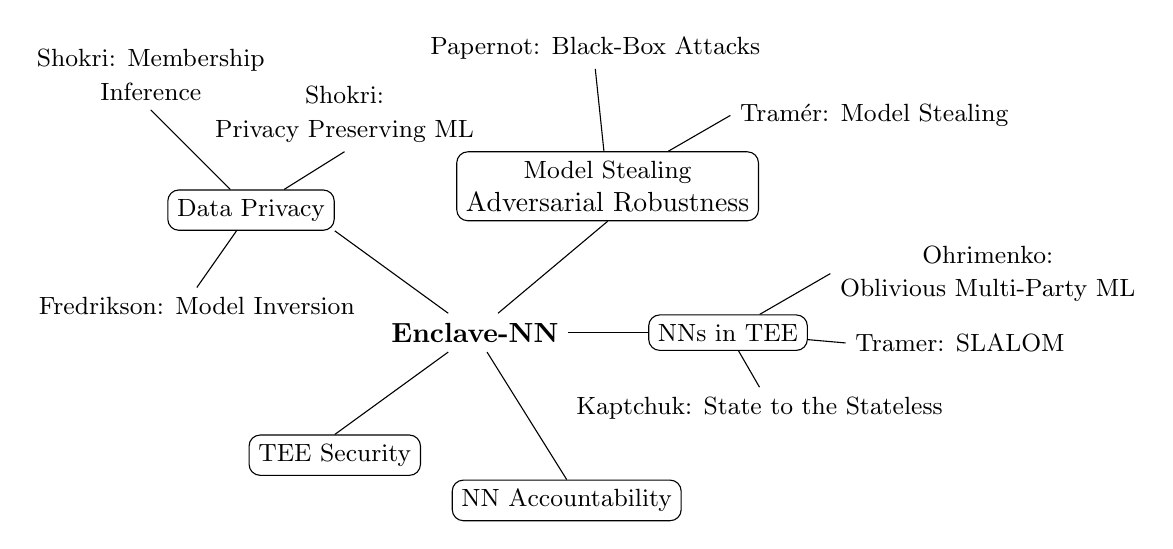
\begin{tikzpicture}
      \node at (0,0) (enclave-nn) {\textbf{Enclave-NN}};

      \draw (enclave-nn) -- (216:2.2) node[below,draw,rounded corners] (enclave-security) {\small TEE Security};
      \draw (enclave-nn) -- (302:2.2) node[below,draw,rounded corners] (nn-accountability) {\small NN Accountability};

      \draw (enclave-nn) -- (40:2.2) node[above,align=center,draw,rounded corners] (model-stealing) {\small Model Stealing \\ Adversarial Robustness};
      \onslide<2->{
        \draw(model-stealing) -- ++(30:1.8) node[right] (stealing-tramer) {\small Tram\'er: Model Stealing};
        \draw(model-stealing) -- ++(96:1.5) node[above] (adv-papernot) {\small Papernot: Black-Box Attacks};
      }
      
      \draw (enclave-nn) -- (0:2.2) node[right,draw,rounded corners] (nn-enclave) {\small NNs in TEE};
      \onslide<3->{
        \draw (nn-enclave) -- ++(30:1.5) node[right, align=center] {\small Ohrimenko:\\ \small Oblivious Multi-Party ML};
        \draw (nn-enclave) -- ++(300:0.8) node[below] {\small Kaptchuk: State to the Stateless};
        \draw (nn-enclave) -- ++(-5:1.5) node[right] {\small Tramer: SLALOM};
      }
      
      \draw (enclave-nn) -- (144:2.2) node[above left,draw,rounded corners] (data-privacy) {\small Data Privacy};
      \onslide<4->{
        \draw (data-privacy) -- ++(32:1.4) node[above,align=center] {\small Shokri:\\\small Privacy Preserving ML};
        \draw (data-privacy) -- ++(135:1.8) node[above,align=center] {\small Shokri: Membership\\\small Inference};
        \draw (data-privacy) -- ++(235:1.2) node[below] {\small Fredrikson: Model Inversion};
      }
    \end{tikzpicture}
  \end{center}
  \vfill
\end{frame}

\begin{frame}
  \frametitle{Stealing Machine Learning Models via Prediction APIs}
  \framesubtitle{\small Tramèr et al. USENIX Security, 2016.}
  \begin{block}{Goal}
    Steal models from prediction API black-boxes
  \end{block}
  \pause
  Approach:
  \begin{enumerate}
  \item Build surrogate model, guessing target architecture
  \item Build starting dataset, getting labels from target
  \item \label{stealing-train}Train surrogate model
  \item Generate synthetic inputs at areas of low confidence
  \item Got to \ref{stealing-train} if not done
  \end{enumerate}
  \pause
  \begin{alertblock}{Relation to Enclave-NN}
    Main attack we have to defend against.\\
    Requires $100 \cdot k$ queries for $k$ parameters, infeasible with rate limiting.
  \end{alertblock}
\end{frame}

\begin{frame}
  \frametitle{Practical Black-Box Attacks against Machine Learning}
  \framesubtitle{\small Papernot et al. ACM, 2017.}
  \begin{block}{Goal}
    Create adversarial examples for black box ML models
  \end{block}
  \pause
  Apprach:
  \begin{itemize}
  \item Send some inputs to target, observe confidence
  \item Train surrogate model on confidence vectors
  \item Adaptively build new inputs based on surrogate's gradients
  \item Create adversarial examples on surrogate model
  \end{itemize}
  \pause
  \begin{alertblock}{Relation to Enclave-NN}
    The current version is more vulnerable than online oracles.\\
    This can be fixed by combining other methods.
  \end{alertblock}
\end{frame}

\againframe<2>{related}

\begin{frame}
  \frametitle{Giving State to the Stateless}
  \framesubtitle{\small Kaptchuk et al. NDSS, 2019}
  \begin{block}{Goal}
    Allow TEE to preserve state between executions
  \end{block}
  \pause
  Approach:
  \begin{itemize}
  \item All inputs go through server
  \item Server keeps ledger of inputs
  \item TEE gets relevant parts of ledger from server
  \item TEE can verify signature and reject invalid inputs
  \end{itemize}
  \pause
  \begin{alertblock}{Relation to Enclave-NN}
    We could use this to implement rate-limiting.\\
    Also required for monetization.
  \end{alertblock}
\end{frame}

\begin{frame}
  \frametitle{SLALOM}
  \framesubtitle{\small Tram\'er and Boneh. arXiv preprint, 2018}
  \begin{block}{Goal}
    Provide integrity and data privacy for ML
  \end{block}
  \pause
  Approach:
  \begin{itemize}
  \item Start model execution in the enclave
  \item Apply additive cipher to input to keep it from leaking
  \item Outsource individual layers to the GPU from enclave
  \item Statistically verify all GPU results
  \end{itemize}
  \pause
  \begin{alertblock}{Relation to Enclave-NN}
    Their focus is on data privacy, ours on model privacy.\\
    The integrity check can be used to build authenticity.
  \end{alertblock}
\end{frame}

\begin{frame}
  \frametitle{Multi-Party Machine Learning on Trusted Processors}
  \framesubtitle{\small Ohrimenko et al. USENIX, 2016.}
  \begin{block}{Goal}
    Allow multiple parties to train collaborative model on private date
  \end{block}
  \pause
  \begin{itemize}
  \item Run Enclave on third-party cloud provider
  \item Send encrypted training data to provider
  \item Provider trains model
  \item Download encrypted model
  \end{itemize}
  \pause
  \begin{alertblock}{Relation to Enclave-NN}
    Final download of encrypted model similar to our approach.\\
    Entire training and inference happens in enclave.\\
    We should have much smaller performance impact.
  \end{alertblock}
\end{frame}

\againframe<3>{related}

\begin{frame}
  \frametitle{Privacy Preserving Deep Learning}
  \framesubtitle{\small Shokri and Shmatikov. ACM, 2015.}
  \begin{block}{Goal}
    Allow multiple parties to train NN on private data
  \end{block}
  \pause
  Approach:
  \begin{enumerate}
  \item Set up state server, (public) model architecture
  \item \label{download} Download state from server
  \item Run training epoch, calculating weight updates
  \item Send percentage of weight updates to state server
  \item Got to \ref{download} if not done
  \end{enumerate}
  \pause
  \begin{alertblock}{Relation to Enclave-NN}
    We could try and solve the same problem with enclaves.\\
    This has already been done.
  \end{alertblock}
\end{frame}

\begin{frame}
  \frametitle{Membership Inference Attacks}
  \framesubtitle{\small Shokri, et al. IEEE, 2017.}
  \begin{block}{Goal}
    Infer whether an input was in training set or not
  \end{block}
  \pause
  Approach:
  \begin{itemize}
  \item Build a surrogate dataset from target model
  \item Train multiple ``shadow models''
  \item Pass training and non-training inputs to shadow models
  \item Train attack classifier on returned confidence vectors
  \item Run attack classifier on outputs of target model
  \end{itemize}
  \pause
  \begin{alertblock}{Relation to Enclave-NN}
    Could leak information about original dataset, but requires confidence values.\\
    This approach exploits properties of data distribution, which we can't influence.
  \end{alertblock}
\end{frame}

\begin{frame}
  \frametitle{Model Inversion Attacks}
  \framesubtitle{\small Fredrikson et al. ACM, 2015}
  \begin{block}{Goal}
    Extract training inputs from ML models via confidence values
  \end{block}
  \pause
  Approach:
  \begin{enumerate}
  \item Find a point in input size for the target class label
  \item \label{inversion-loop} Move towards area of higher confidence
  \item De-noise image
  \item Go to \ref{inversion-loop} if not done
  \end{enumerate}
  \pause
  \begin{alertblock}{Relation to Enclave-NN}
    Requires confidence values, which we would not return.\\
    Our model would not be easily differintable.
  \end{alertblock}
\end{frame}

\againframe<4>{related}

\section{Future Work}
\begin{frame}
  \frametitle{Future Work}
  \begin{itemize}
  \item Inference on private data without encryption
  \item More general Enclave code and loading weights
  \item Validation/Authentication of predictions
  \item Automatic Enclave compilation
  \end{itemize}
\end{frame}

\end{document}
